              %******************************************%
              %                                          %
              %     Modello di articolo scientifico      %
              %            di Luca Benvenuti             %
              %                                          %
              %         versione: 22 maggio 2013         %
              %                                          %
              %******************************************%
       

% I seguenti commenti speciali impostano:
% 1. utf8 come codifica di input,
% 2. PDFLaTeX come motore di composizione;
% 3. Articolo.tex come documento principale;
% 4. il controllo ortografico italiano per l'editor.

% !TEX encoding = UTF-8
% !TEX TS-program = pdflatex
% !TEX root = Articolo.tex
% !TEX spellcheck = it-IT

\documentclass[12pt,%                       % corpo del font principale
               a4paper,%                    % carta A4
              oneside,%                    % solo fronte
           %   twoside,%                    % fronte-retro
               ]{article}                  % classe report di KOMA-Script;
	   
			   
\usepackage{fancyhdr}
               
\usepackage[T1]{fontenc}                    % codifica dei font:
                                            % NOTA BENE! richiede una distribuzione *completa* di LaTeX,
                                          % per esempio TeXLive o MiKTeX *complete*

\usepackage[utf8]{inputenc}              % codifica di input; anche [latin1] va beneutf8
                                           % NOTA BENE! va accordata con le preferenze dell'editor


\usepackage{microtype}                     % microtipografia

\usepackage[italian,english]{babel}        % per scrivere in italiano e in inglese;
                                           % l'ultima lingua (l'italiano) risulta predefinita
                                           
\usepackage[binding=5mm]{layaureo}         % margini ottimizzati per l'A4; rilegatura di 5 mm


\usepackage{lmodern}  					   %new gerahrd
\usepackage{cleveref}  					   %new gerahrd
\usepackage{emptypage}     
\usepackage{indentfirst}                    % rientra il primo capoverso di ogni sezione

\usepackage{booktabs}                       % tabelle
\usepackage{tabularx}                       % tabelle di larghezza prefissata
\usepackage{graphicx}                       % immagini

\usepackage{subfig}                         % sottofigure, sottotabelle
\usepackage{caption}                        % didascalie

\usepackage{listings}                       % codici

\usepackage[font=small]{quoting}            % citazioni

\usepackage{amsmath,amssymb,amsthm}        % matematica
\usepackage{amsxtra,amstext,amsfonts}
\usepackage{amscd}						   %chimica

\usepackage[english]{varioref}              % riferimenti completi della pagina

\usepackage{mparhack,fixltx2e,relsize}      % finezze tipografiche
\usepackage[babel]{csquotes}
      
\usepackage[style=numeric-comp,hyperref,backref,backend=bibtex]{biblatex}
\bibliography{Bibliografia}                 % database di biblatex 
                                          
\usepackage{chngpage,calc}                 % centra il frontespizio
\usepackage[dvipsnames]{xcolor}             % colori
\usepackage{color}

\usepackage{lipsum}                        % testo fittizio

\usepackage{eurosym}                       % simbolo dell'euro

\usepackage[pdfa]{hyperref}                      % collegamenti ipertestuali

\usepackage{bookmark}                      % segnalibri
\usepackage[figuresright]{rotating}

\usepackage{array}

\usepackage{enumitem}

\usepackage{colortbl}

\usepackage{floatflt}
\usepackage{titlesec}

\usepackage{eurosym}  %indovina

\setcounter{tocdepth}{5} %to make it appears in TOC
\setcounter{secnumdepth}{5} %to make it numbered


\usepackage{acronym}
\usepackage{rotating}

%*********************************************************************************
% impostazioni-articolo.tex
% di Lorenzo Pantieri (2012)
% file che contiene le impostazioni dell'articolo
%*********************************************************************************


%*********************************************************************************
% Comandi personali
%*******************************************************
%\newcommand{\myName}{Lorenzo Pantieri}                            % autore
\newcommand{\myTitle}{Characterization of Particle Based Simulation Parameters
by means of Artificial Neural Networks}  % titolo
\date{}                                                           % nessuna data

%\title{\myTitle}
%\author{\myName}



%*********************************************************************************
% Impostazioni di amsmath, amssymb, amsthm
%*********************************************************************************

% comandi per gli insiemi numerici (serve il pacchetto amssymb)
\newcommand{\numberset}{\mathbb} 
\newcommand{\N}{\numberset{N}} 
\newcommand{\R}{\numberset{R}} 

% un ambiente per i sistemi
\newenvironment{sistema}%
  {\left\lbrace\begin{array}{@{}l@{}}}%
  {\end{array}\right.}

% definizioni (serve il pacchetto amsthm)
\theoremstyle{definition} 
\newtheorem{definizione}{Definizione}

% teoremi, leggi e decreti (serve il pacchetto amsthm)
\theoremstyle{plain} 
\newtheorem{teorema}{Teorema}
\newtheorem{legge}{Legge}
\newtheorem{decreto}[legge]{Decreto}
\newtheorem{murphy}{Murphy}[section]



%*********************************************************************************
% Impostazioni di biblatex
%*********************************************************************************
\defbibheading{bibliography}{%
\phantomsection
\addcontentsline{toc}{section}{\refname}
\section*{\bibname\markboth{\MakeUppercase{\refname}}{\MakeUppercase{\refname}}}}



%*********************************************************************************
% Impostazioni di listings
%*********************************************************************************
\lstset{language=[LaTeX]Tex,%C++,
    keywordstyle=\color{RoyalBlue},%\bfseries,
    basicstyle=\small\ttfamily,
    %identifierstyle=\color{NavyBlue},
    commentstyle=\color{Green}\ttfamily,
    stringstyle=\rmfamily,
    numbers=none,%left,%
    numberstyle=\scriptsize,%\tiny
    stepnumber=5,
    numbersep=8pt,
    showstringspaces=false,
    breaklines=true,
    frameround=ftff,
    frame=single
} 



%*********************************************************************************
% Impostazioni di hyperref
%*********************************************************************************
% \hypersetup{%
%     hyperfootnotes=false,pdfpagelabels,
%     %draft,	% = elimina tutti i link (utile per stampe in bianco e nero)
%     colorlinks=true, linktocpage=true, pdfstartpage=1, pdfstartview=FitV,%
%     % decommenta la riga seguente per avere link in nero (per esempio per la stampa in bianco e nero)
%     %colorlinks=false, linktocpage=false, pdfborder={0 0 0}, pdfstartpage=1, pdfstartview=FitV,% 
%     breaklinks=true, pdfpagemode=UseNone, pageanchor=true, pdfpagemode=UseOutlines,%
%     plainpages=false, bookmarksnumbered, bookmarksopen=true, bookmarksopenlevel=1,%
%     hypertexnames=true, pdfhighlight=/O,%nesting=true,%frenchlinks,%
%     urlcolor=webbrown, linkcolor=RoyalBlue, citecolor=webgreen, %pagecolor=RoyalBlue,%
%     %urlcolor=Black, linkcolor=Black, citecolor=Black, %pagecolor=Black,%
%     pdftitle={\myTitle},%
%     pdfauthor={\textcopyright\ \myName},%
%     pdfsubject={},%
%     pdfkeywords={},%
%     pdfcreator={pdfLaTeX},%
%     pdfproducer={LaTeX with hyperref and ClassicThesis}%
% }



%*********************************************************************************
% Impostazioni di graphicx
%*********************************************************************************
%\graphicspath{{Immagini/}} % cartella dove sono riposte le immagini



%*********************************************************************************
% Impostazioni di xcolor
%*********************************************************************************
\definecolor{webgreen}{rgb}{0,.5,0}
\definecolor{webbrown}{rgb}{.6,0,0}



%*********************************************************************************
% Impostazioni di caption
%*********************************************************************************
\captionsetup{tableposition=top,figureposition=bottom,font=small,format=hang,labelfont=bf}



%*********************************************************************************
% Altro
%*********************************************************************************

% [...] ;-)
\newcommand{\omissis}{[\dots\negthinspace]}

% eccezioni all'algoritmo di sillabazione
\hyphenation{Fortran ma-cro-istru-zio-ne nitro-idrossil-amminico}

\pagenumbering{gobble} %to switch off page numbering.               % file con le impostazioni personali



\begin{document}
\pagestyle{headings} 
%******************************************************************
% Materiale iniziale
%******************************************************************
% !TEX encoding = UTF-8
% !TEX TS-program = pdflatex
% !TEX root = ../Articolo.tex
% !TEX spellcheck = it-IT

%*******************************************************
% Frontespizio
%*******************************************************
\begin{titlepage}
\pdfbookmark{Frontespizio}{Frontespizio}
\changetext{}{}{}{((\paperwidth - \textwidth) / 2) - \oddsidemargin - \hoffset - 1in}{}

\begin{center}


% Upper part of the page

\includegraphics[width=0.3\textwidth]{045PFM_Logo_Original}\\[1cm]    

\textsc{\LARGE \myDepartment}\\[1.5cm]


% This document uses the following counting scheme
%    I   - Year for Q1 of the year Year
%    II  - Year ...
%    III - Year
%    IV  - Year
\textsc{\Large \myTitle ~ - \RM{8}  - 2015}\\[0.5cm]


% Title
\HRule \\[0.4cm]
{ \huge \bfseries \myPhd}\\[0.4cm]

\HRule \\[1.5cm]

% Author and supervisor

\begin{minipage}{0.8\textwidth}
\begin{center} \large

\emph{Author:}\\[0.4cm]

%irstname \textsc{Lastname}
\myName \\
\texttt{\myemail}\\[1.5cm]

\emph{Supervisors:} \\[0.4cm]

\myProf \\[0.2cm]
\myOtherProf \\ [0.2cm]
%\end{flushright}

\end{center}

\end{minipage}

\vfill

% Print the current date at the bottom of the page
{\large \myTime}

\end{center}

\end{titlepage}

% !TEX encoding = UTF-8
% !TEX TS-program = pdflatex
% !TEX root = ../Articolo.tex
% !TEX spellcheck = it-IT

%*******************************************************
% Indici
%*******************************************************
\pdfbookmark{\contentsname}{tableofcontents}
\setcounter{tocdepth}{2}
\tableofcontents
\markboth{\contentsname}{\contentsname} 

%*******************************************************
% Elenco delle figure
%*******************************************************    
\phantomsection
\pdfbookmark{\listfigurename}{lof}
\listoffigures

%*******************************************************
% Elenco delle tabelle
%*******************************************************
\phantomsection
\pdfbookmark{\listtablename}{lot}
\listoftables
       
	   
\newpage
%
%% !TEX encoding = UTF-8
% !TEX TS-program = pdflatex
% !TEX root = ../Articolo.tex
% !TEX spellcheck = it-IT

%*******************************************************
% Sommario+Abstract
%*******************************************************
\phantomsection
\pdfbookmark{Sommario}{Sommario}
\section*{Sommario}

\lipsum[1]

\selectlanguage{english}
\pdfbookmark{Abstract}{Abstract}
\section*{Abstract}

\lipsum[2]

\selectlanguage{italian}


%******************************************************************
% Materiale principale
%******************************************************************

% !TEX encoding = UTF-8
% !TEX TS-program = pdflatex
% !TEX root = ../Tesi.tex
% !TEX spellcheck = en-EN

%************************************************
\part{Introduction}
\label{par:introduction}
%************************************************

Particles in various forms - ranging from raw materials to food grains and pharmaceutical powders - 
play a major role in a variety of industries, including process industry and metallurgy. 
In his book, \citet{RefWorks:117} stated that "between 1 and 10\% of all the energy is used in 
comminution, i.e. the processes of crushing, grinding, milling, micronising". 
Many methods have been developed to study particles.
For instance, Discrete Element Methods ($DEMs$), "a special class of numerical
schemes for simulating the behavior of discrete, interacting bodies", are widely used to 
simulate particle behaviour in these granular processes
(\citet{RefWorks:130}).\\ 
\begin{figure}[!htb]
\centering
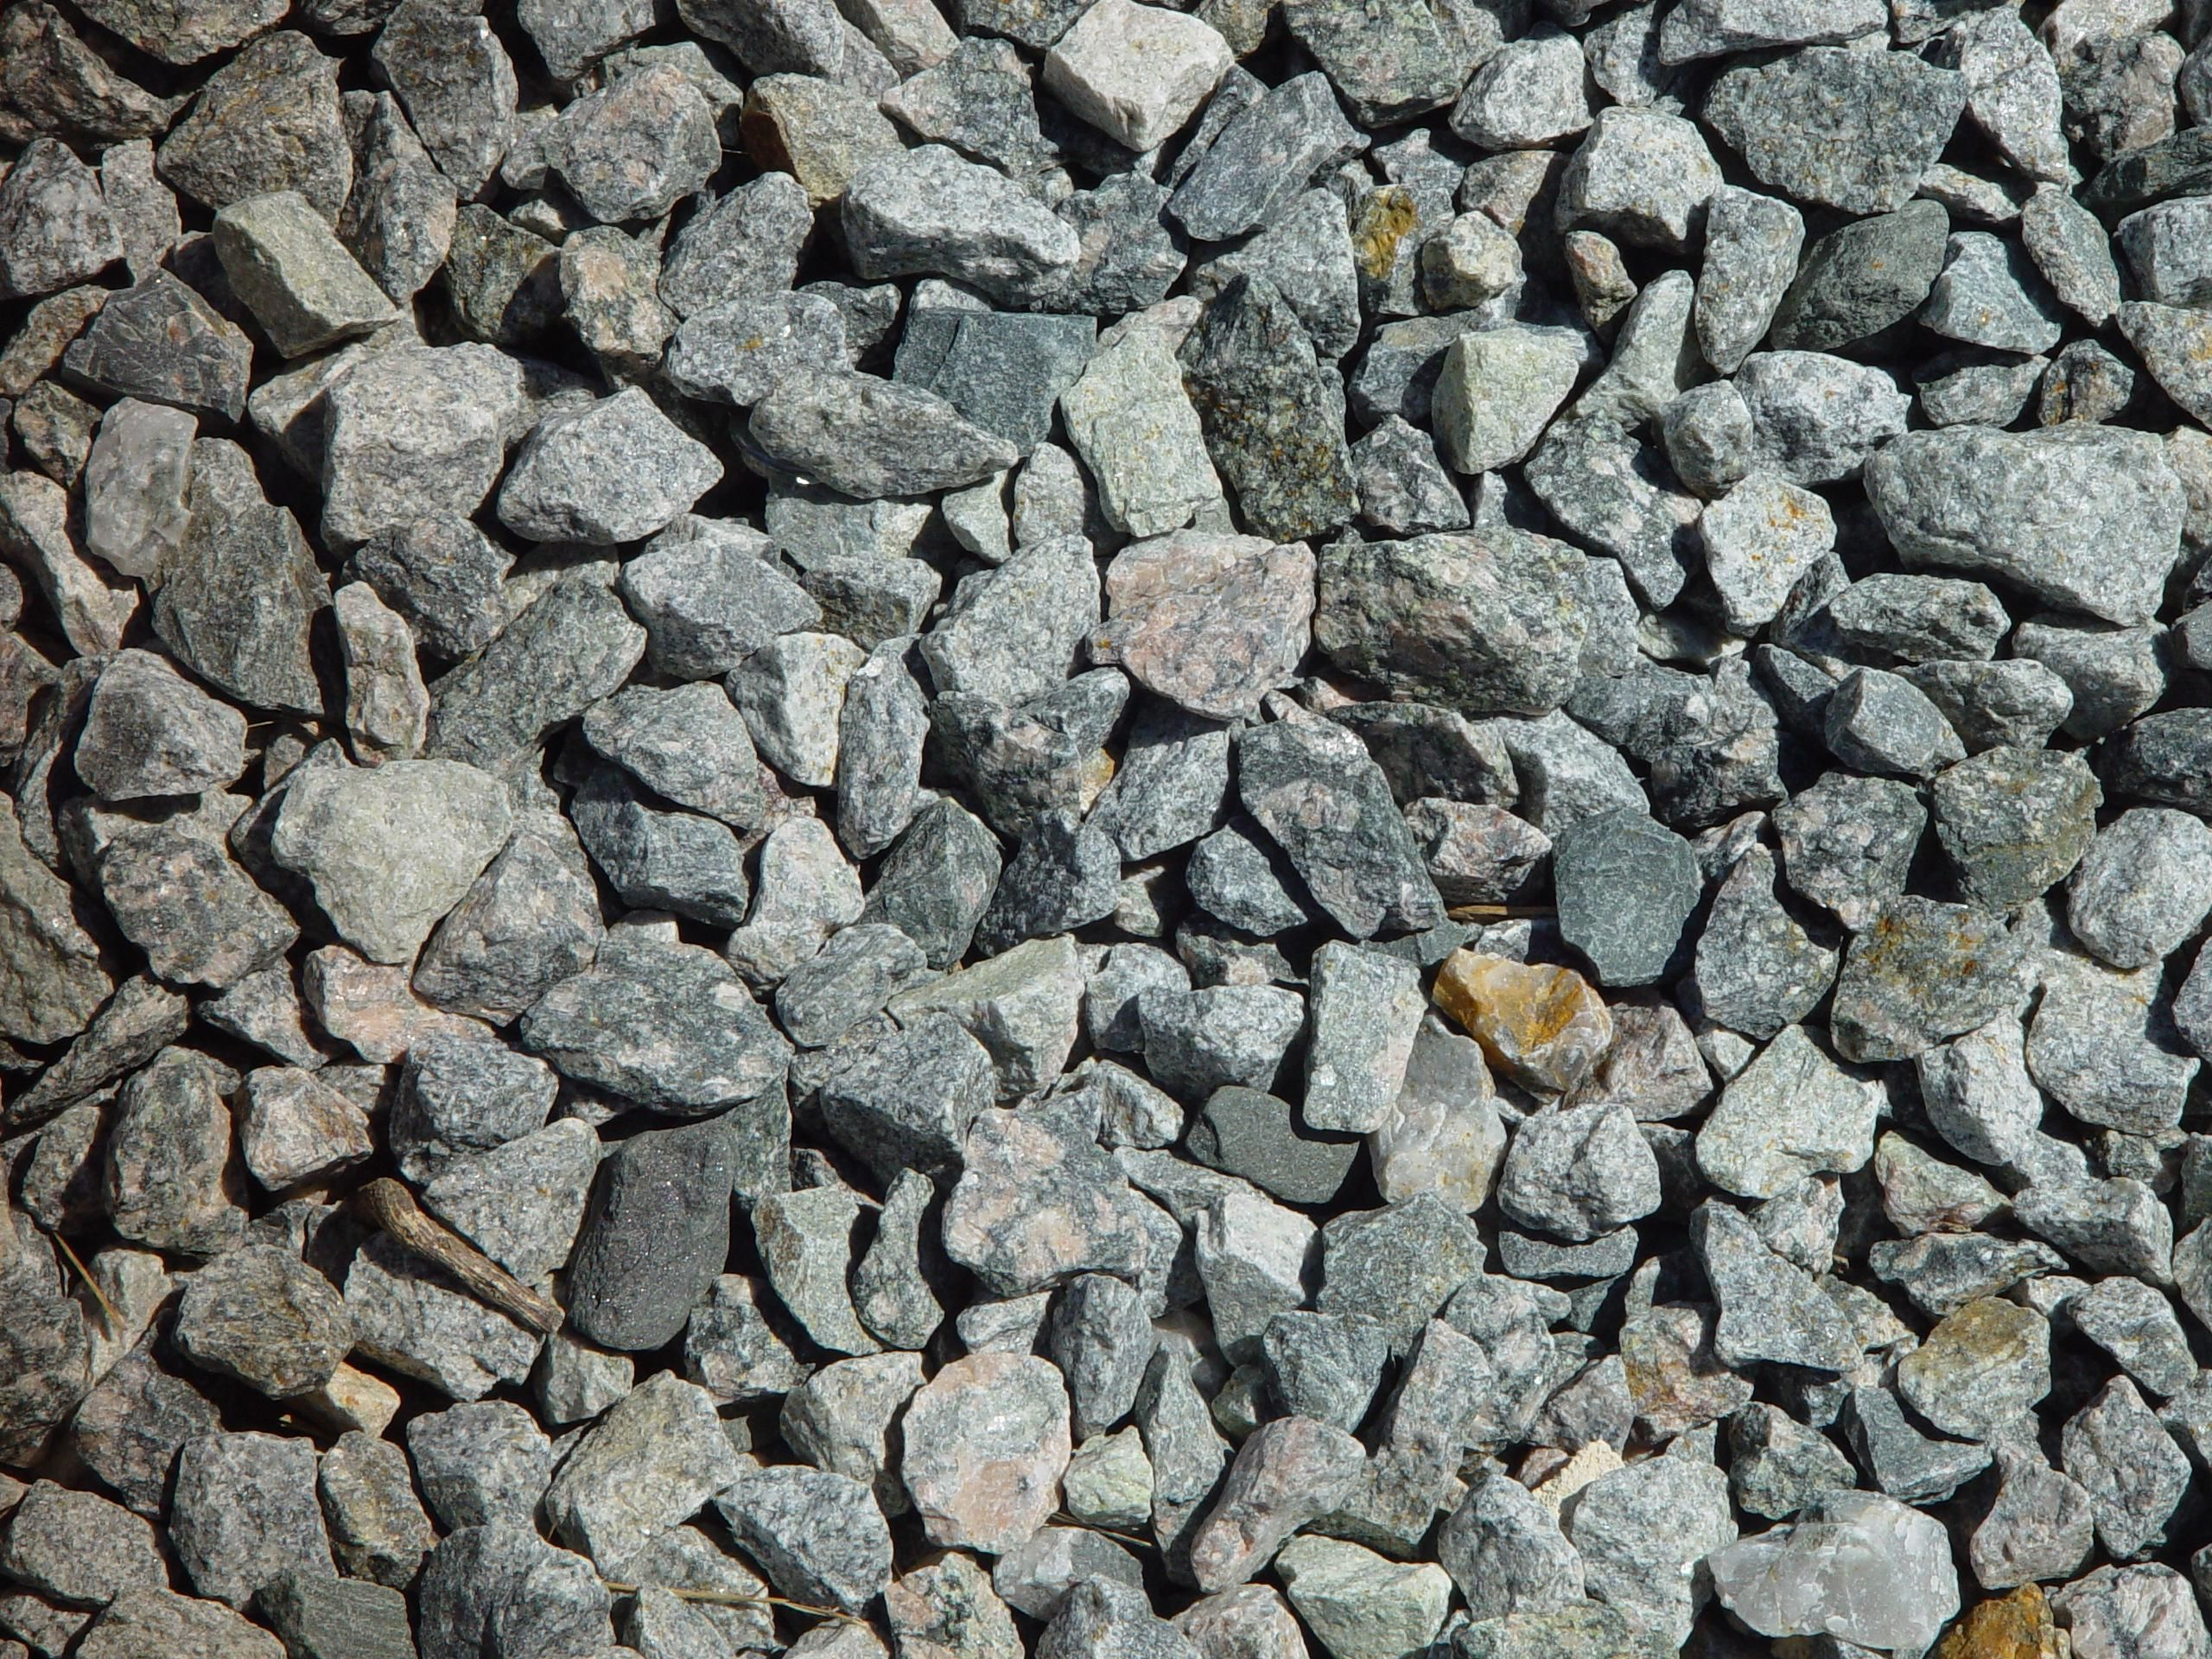
\includegraphics[width=.50\columnwidth]{images/133gravel}
\caption[Gravel]{Gravel.}
\label{fig:133gravel}
\end{figure}
\begin{figure}[!htb]
\centering
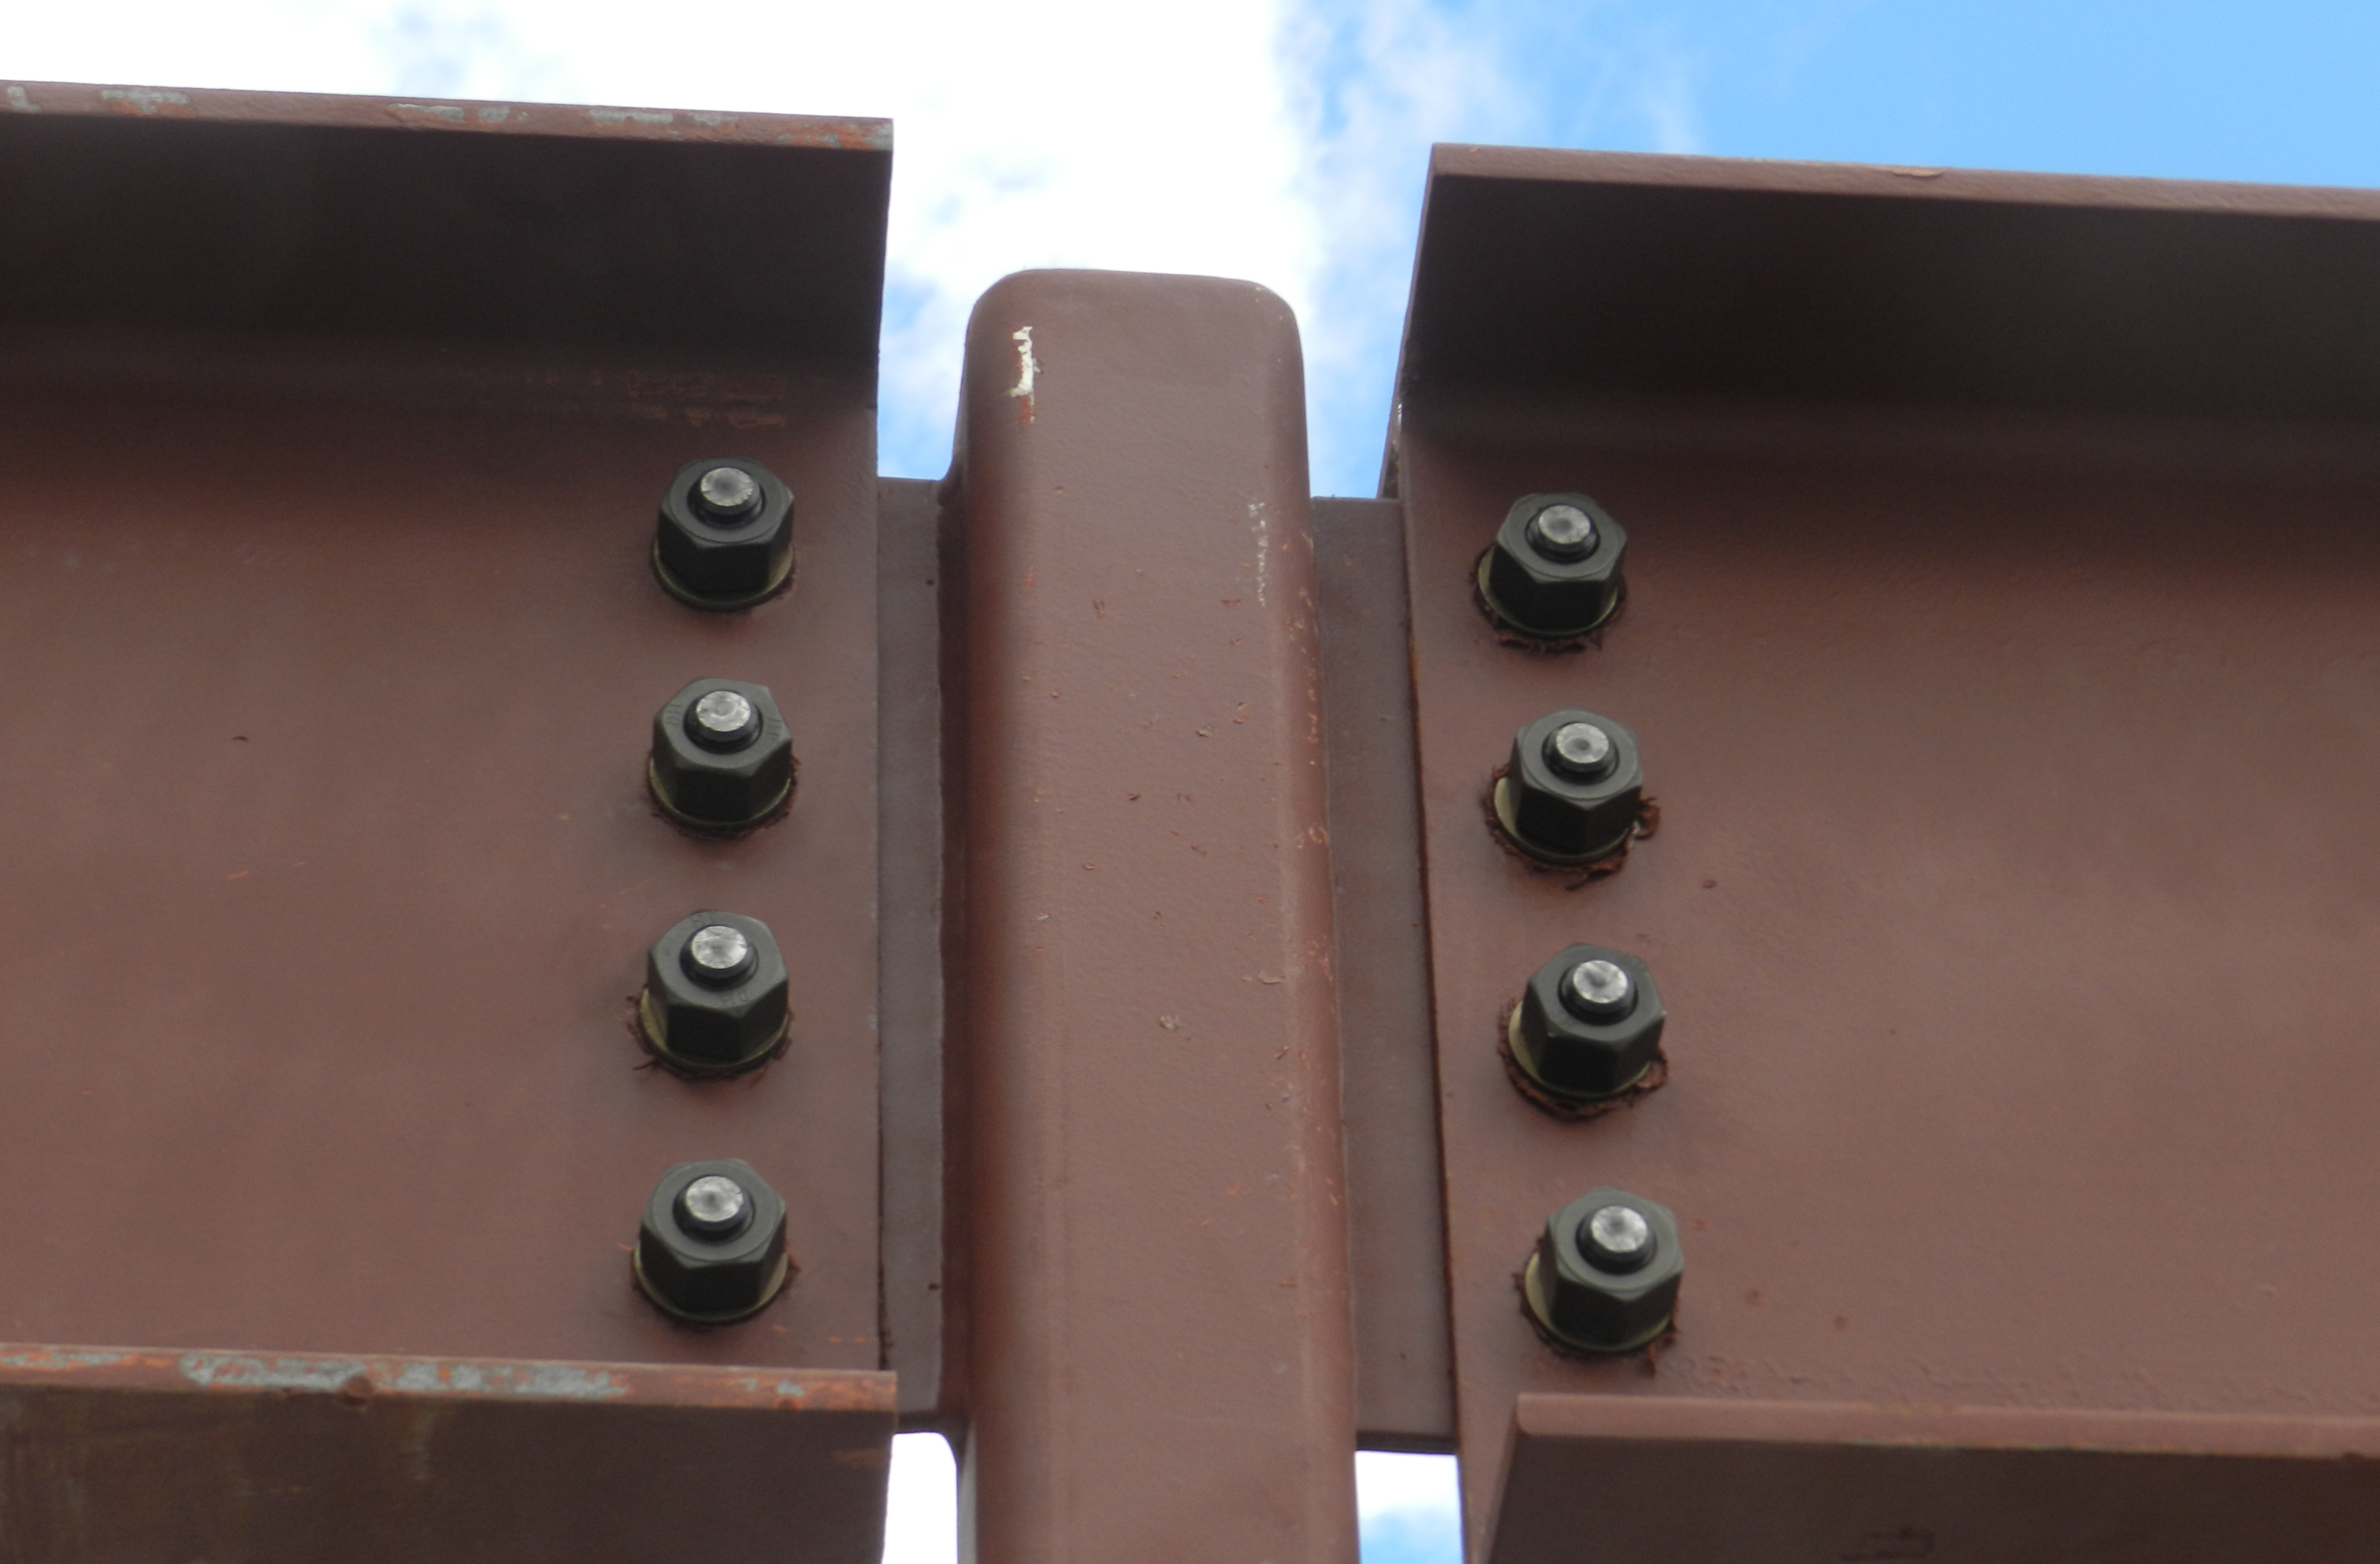
\includegraphics[width=.50\columnwidth]{images/050steel}
\caption[Steel]{Steel.}
\label{fig:050steel}
\end{figure}
In fact, gravels, Fig. \ref{fig:054bsgmaterials}, or granular particles in
general, are far from being a well-defined and easy to characterize material,
for instance a steel beam, Fig.
\ref{fig:050steel}. For continuous materials simulation
parameters are readily available.
In case of a pile of particles the sum of discrete particle properties determines the pile's macroscopic behavior 
(e.g. angle of repose).
In discrete particle simulations particle based parameters (e.g. contact parameters) determine the macroscopic behavior 
of the ensemble.
Unfortunately, particles are not uniform and particle based simulation
parameters are difficult to obtain, and also depends on the numerical shape
(polyhedral, multi-spheres, and simple spheres).
A set of experimental and numerical solutions, together with artificial neural networks, can improve the accuracy 
and the range of applicability of the characterization of particles properties, and reduce the computational costs.
Discrete Element Method requires parameters for the individual contact, but characterize every particle is prohibitive.
We need to find average contact parameters that lead to the expected bulk effect.
We could start with an example of piled particles, more specifically called the
drained angle of repose. This angle of repose \ref{fig:060aor},
characteristic of the bulk macroscopic behaviour of the ensemble, is originated from the microscopic
characteristics of each particle.
\begin{figure}[htbp]
  %\null\hfill
  \subfloat[Silibeads angle of repose.]{
	  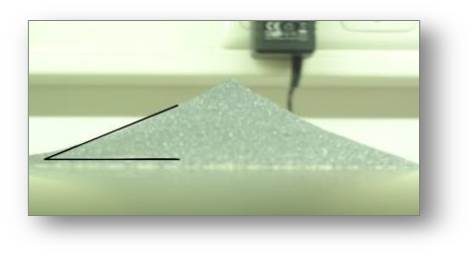
\includegraphics[width=.48\columnwidth]{images/058silibeads}
	  \label{fig:058silibeads}
  }
  \quad
 % \hfill
  \subfloat[Sinter pellets  angle of repose.]{
	  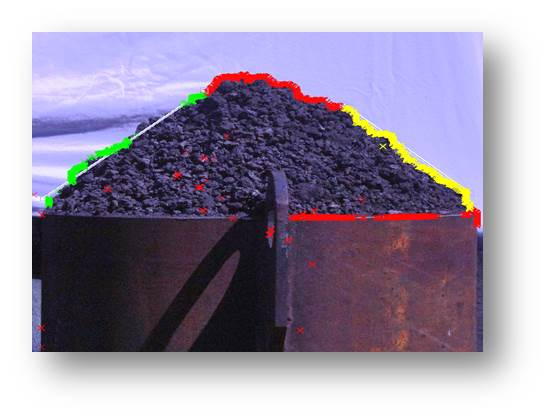
\includegraphics[width=.48\columnwidth]{images/059sinterpellets}
	  \label{fig:059sinterpellets}
  }
 % \hfill\null
  \caption{Angle of repose identification.}
  \label{fig:060aor}
\end{figure}
Measurement of a bulk parameter value, through calibration we obtain the
individual contact parameters:
\begin{enumerate}
\item{Chose initial set of parameters}
\item{DEM simulation}
\item{Compare macroscopic DEM simulation results with experiments}
\item{Choose new parameters}
\end{enumerate}
By our calibration procedure we obtain valid sets of particle based simulation parameters.
Ok, but that's very time consuming, because in each control loop we have to
perform a complete $DEM$ simulation in our case we would need 9.900 days on a 32
core machine. It is not necessary to evaluate a huge number of parameter sets,
rather we should try to evaluate the \textbf{sensitivity} 
of the macroscopic bulk behavior with respect to individual particle based parameters.
This can be realized efficiently by artificial neural networks Fig.
\ref{fig:048neuron0}!
\improvement{few words on biological relationship}
\begin{figure}[!htb]
\centering
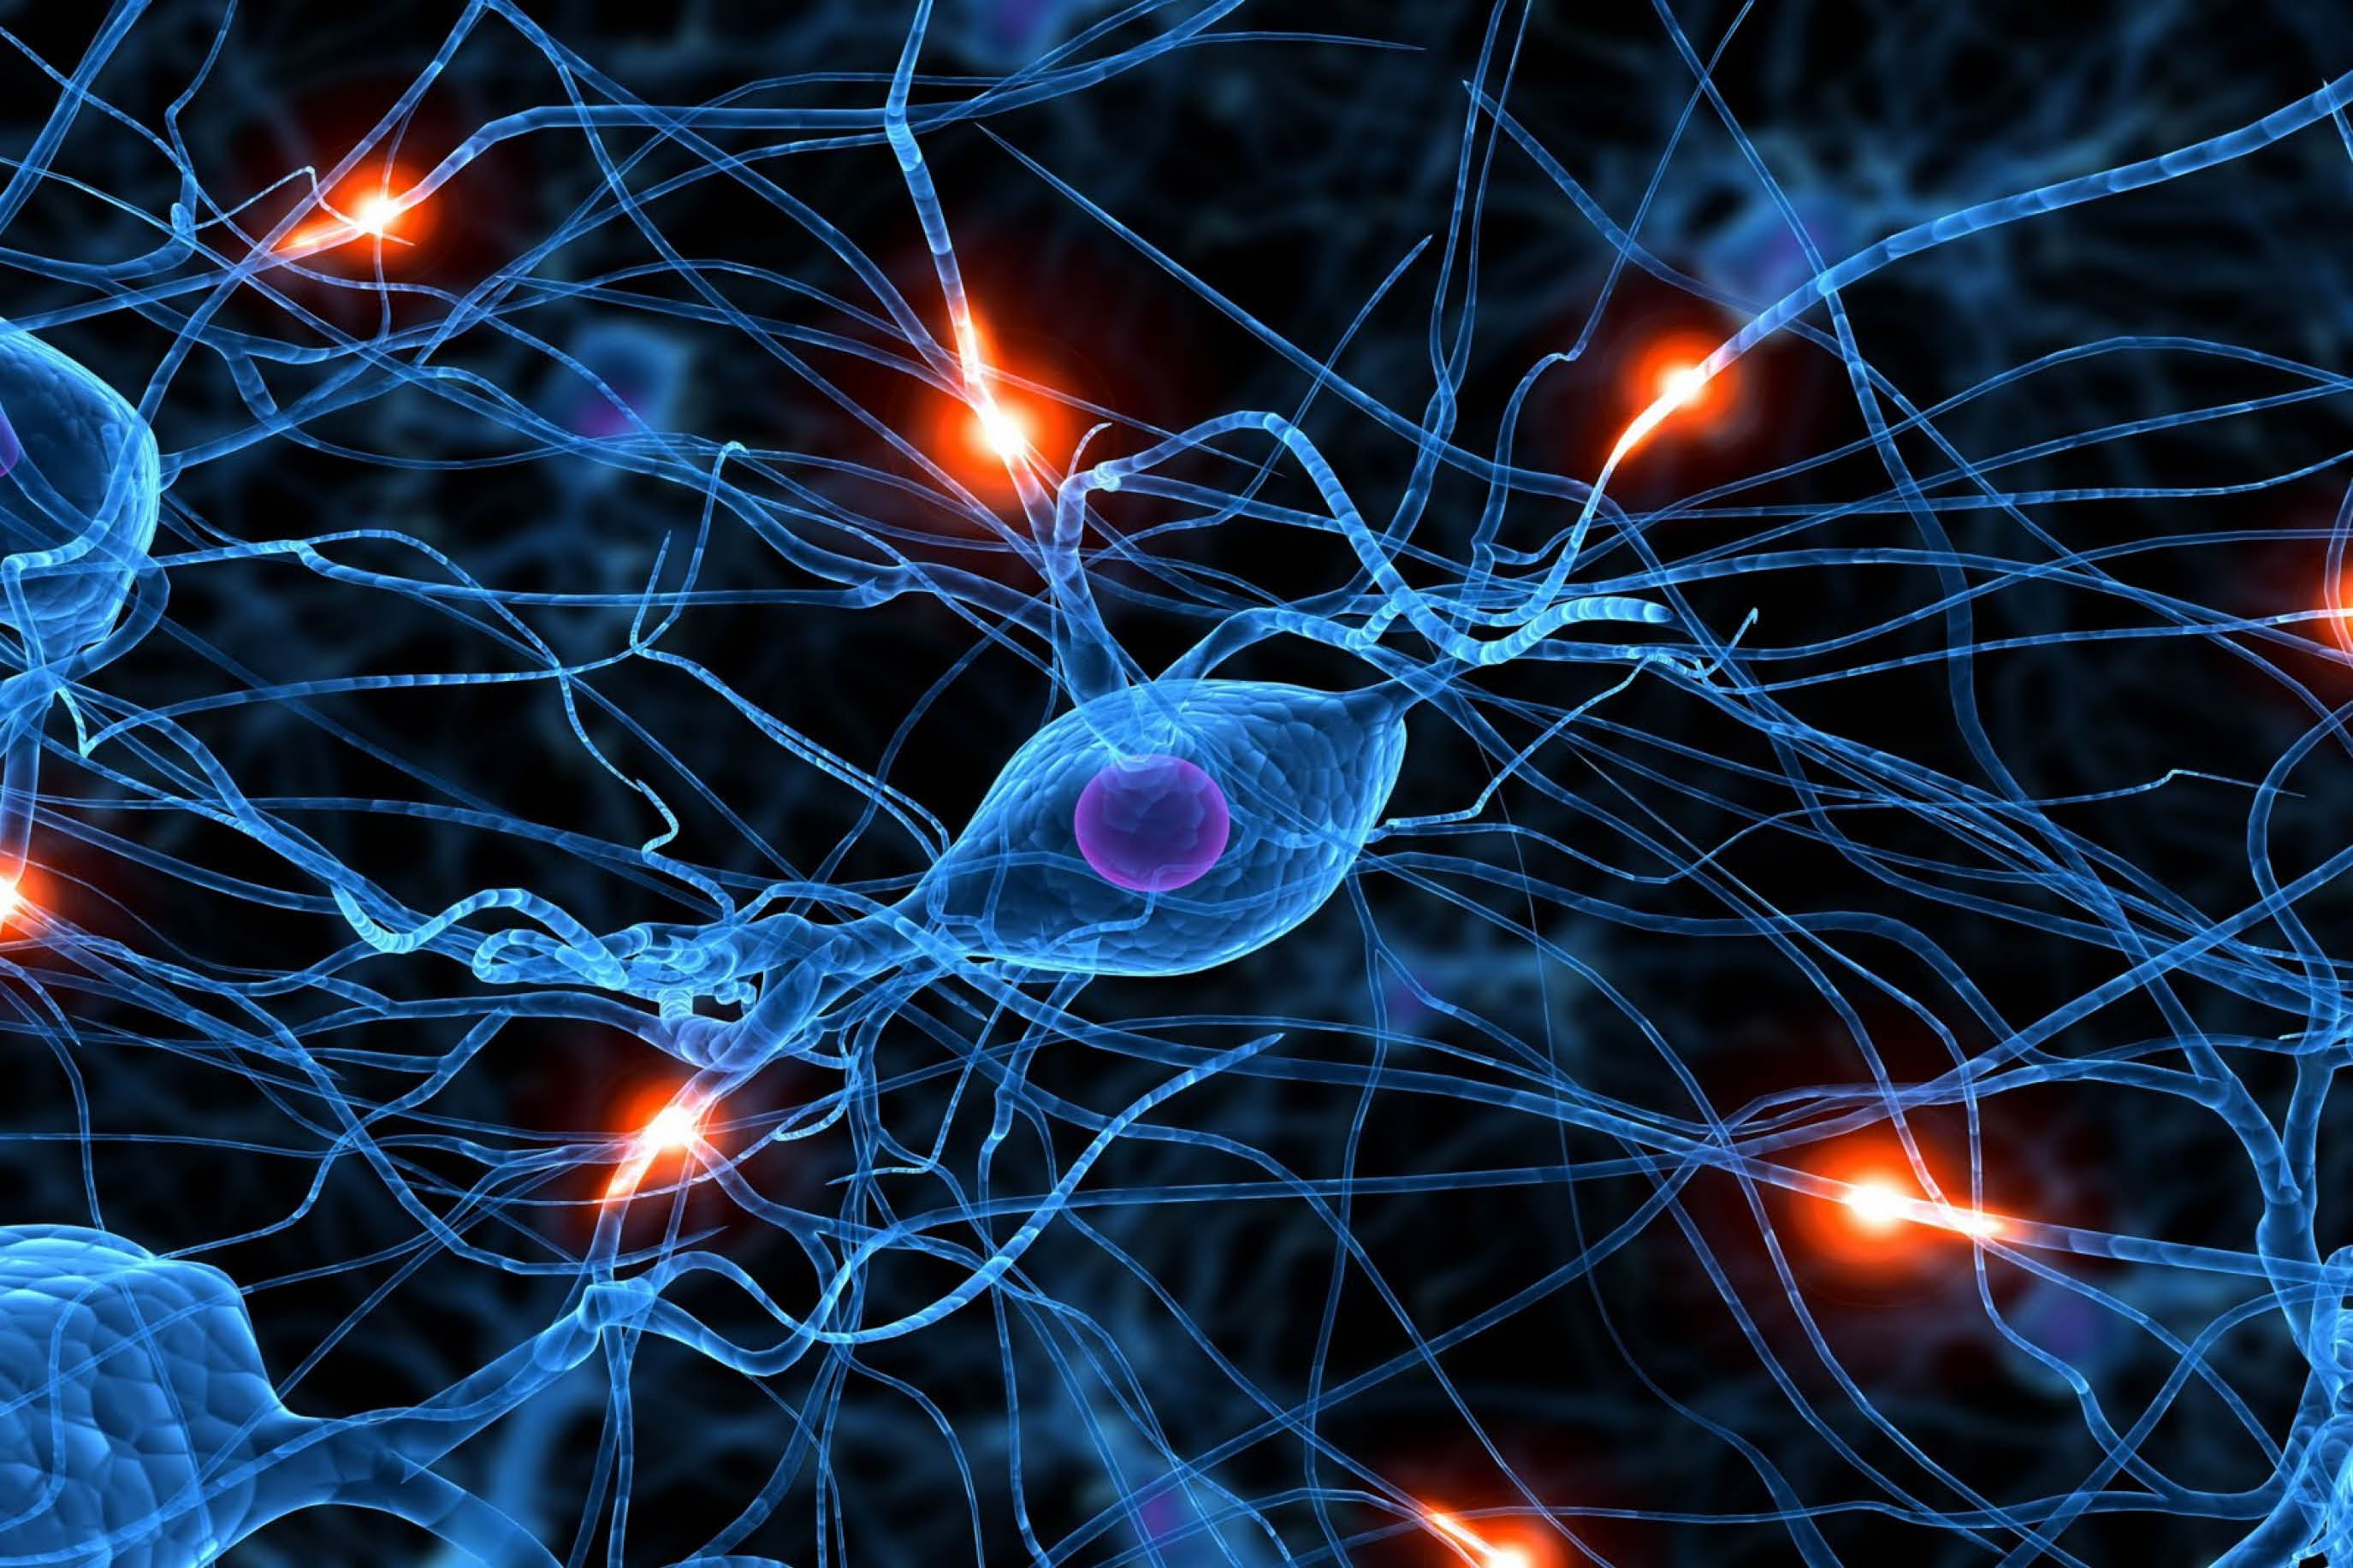
\includegraphics[width=.50\columnwidth]{images/048neuron0}
\caption[Biological inspiration]{Biological inspiration for the Artificial
Neural Networks: a human neuron with the incoming electric signals
\cite{RefWorks:158}.}
\label{fig:048neuron0}
\end{figure}
In this artificial neural network neurons are linked to particle based input parameters. 
By matching the output of the artificial neural network to DEM simulation results the network is trained 
(i.e. individual neurons are weighted).
Later, the trained neural network can be used to predict additional valid sets of particle based simulation parameters. 

\begin{enumerate}
\item{Train neural network by 500 dedicated DEM simulations (time consuming)}
\item{Test another 6.250.000 combinations by the neural network (very fast)}
\item{Check if predictions of neural network are correct (by comparing with experimental  values)}
\end{enumerate}

Typically, less than 1\% of the tested parameter sets lead to correct
macroscopic results (i.e. 6.000 to 60.000 valid parameter sets).
By this assessment of particle based simulation parameters we obtain valuable information about the dependence 
of bulk solid behavior on individual particle properties.
First we can determine the validity range, mean and variance band of each input
parameter. Next we can determine a probability density function for each input
parameter. Then, we can investigate mutual dependencies.
This calibration procedure is universal in a sense that the same artificial neural network can be harnessed for 
different macroscopic bulk behaviors.
This effort is really necessary because the predictive capability of any DEM simulation strongly 
depends on the validity of the particle 
based simulation parameters.
\improvement{add some words on the applications}

% !TEX encoding = UTF-8
% !TEX TS-program = pdflatex
% !TEX root = ../Articolo.tex
% !TEX spellcheck = it-IT

%************************************************
\section{Methodology}
\label{section:methodology}
%************************************************

Two regions were created: porous and air.
The porous region was a parallelepiped with a quadratic base and an height of
1.15 m in the z axis. The base edge was 0.14 m, making the base area
equivalent to the experimental one.
The air region had the same base of the porous region, but had an height of
1.35 m.
From $z=0.1 ~m$ to $z=1.25 ~m$ the two regions shared the same volume.\\
The solver used is \textbf{chtMultiRegionSimpleFoam}, since we had a steady hot
air flow as lower boundary condition, hence a steady state solver.
The solver consider the fluid region as compressible flow.\\
A series of probes, as indicated by \textcite{RegionProbe}, were positioned to
register the temperature.

\subsection{Permeability coefficient}
\label{subsection:permeabilitycoefficient}

The value of the $d$ coefficient has been varied, by order of magnitudes, to
evaluate its effect on the temperature.

\subsection{Flow velocity}
\label{subsection:flowvelocity}

The value of the flow velocity $U$ has been varied to
evaluate its effect on the temperature.

\subsection{Time interval}
\label{subsection:timeinterval}

The total simulation time has been corrected to match the experimental time.
% !TEX encoding = UTF-8
% !TEX TS-program = pdflatex
% !TEX root = ../Articolo.tex
% !TEX spellcheck = it-IT

%************************************************
\section{Results and Discussion}
\label{section:resultsdiscussion}
%************************************************



\subsection{Comparison}
\label{subsection:comparison}

First, the effect of different $\bar{\bar{d}}$ coefficients has been evaluated, see Fig.
\ref{fig:04dvariation}.
It can be seen that the effect for low velocity flow regimes ($U = 0.1 ~m/s$) is
negligible.\\
Later, we selected $\bar{\bar{d}} = 10 ~m^{-2}$, as suggested by
\textcite{Permeability}, and we considered the variation of the flow velocity
$U$.
Since the flow velocity deeply influences the temperature, see Fig.
\ref{fig:05uvariation}, all the simulations in Fig. \ref{fig:04dvariation} were
not further considered.\\
Finally, we performed simulations with the correct duration and temperature, to
evaluate the flow speed in z direction.
It is clear from Fig. \ref{fig:06uvariation2} that the flow velocity $U = 1.5
~m/s$ is the most accurate prediction between those evaluated.

\begin{figure}[!h]
\centering
\subfloat[$\bar{\bar{d}}$ variation, $U = 0.1 ~m/s$]
{\label{fig:04dvariation}%
\includegraphics[width=0.8\columnwidth]{04dvariation}} \\ 
\subfloat[$U$ variation, $\bar{\bar{d}} = 10 ~m^{-2}$]
{\label{fig:05uvariation}%
\includegraphics[width=0.8\columnwidth]{05uvariation}} \\  
\subfloat[$U$ variation, $\bar{\bar{d}} = 10 ~m^{-2}$, experimental comparison]
{\label{fig:06uvariation2}%
\includegraphics[width=0.8\columnwidth]{06uvariation2}} \\  
\caption[Simulations]{Simulations}
\label{fig:simulations}
\end{figure}

\subsection{Temperature variation}
\label{subsection:temperaturevariation}

\begin{figure}[!h]
\centering
\subfloat[t = 25 s]
{\label{fig:0701}%
\includegraphics[height=8cm]{0701}} \quad 
\subfloat[t = 150 s]
{\label{fig:0806}%
\includegraphics[height=8cm]{0806}} \quad  
\subfloat[t = 300 s]
{\label{fig:0912}%
\includegraphics[height=8cm]{0912}} \\  
\subfloat[t = 450 s]
{\label{fig:1018}%
\includegraphics[height=8cm]{1018}} \quad  
\subfloat[t = 600 s]
{\label{fig:1124}%
\includegraphics[height=8cm]{1124}} \\  
\caption[Temperature variations with time]{Temperature variations with time}
\label{fig:simulations2}
\end{figure}

In Fig. \ref{fig:simulations2} we show the variation of temperature with time
during the most accurate simulation ($\bar{\bar{d}} = 10 ~m^{-2}$, $U = 1.5
~m/s$).
In these images the domain is sliced along the z axis, so we can see how the
temperature boundary condition propagates through the domain.

% !TEX encoding = UTF-8
% !TEX TS-program = pdflatex
% !TEX root = ../Tesi.tex
% !TEX spellcheck = en-EN

%************************************************
\part{Conclusion}
\label{par:conclusion}
%************************************************

We have presented a two-step method for $DEM$ simulation parameter
identification. In the first step, an artificial neural network is 
trained using dedicated $DEM$ simulations in order to predict bulk 
behaviours as function of a set of $DEM$ simulation parameters. 
In the second step, this artificial neural network is then used 
to predict the bulk behaviour of a huge number of additional $DEM$ parameter
sets.
The main findings of this study can be summarized as follows:
\begin{itemize}
  \item{An artificial neural network can be trained by a limited number of
  dedicated $DEM$ simulations.
  		The trained artificial neural network is then able to predict
  		granular bulk behaviour.}
  \item{This prediction of granular bulk behaviour is much more efficient
  		than computationally expensive $DEM$ simulations.
  		Thus, the macroscopic output associated with a huge number of parameter sets
  		can be studied.}
  \item{If the predictions of the artificial neural network are compared to a bulk experiment, 
  		valid sets of $DEM$ simulation parameters can be readily deduced for a
  		specific granular material.}
  \item{This $DEM$ parameter identification method can be applied to
  arbitrary bulk experiments.
  		Combining two artificial neural networks which predict two different bulk
  		behaviours leads to winnowing the set of valid $DEM$ simulation parameters.}
\end{itemize}
As part of future work, we will develop this method further by considering
different fractions of granular materials, which will lead to size-dependent sets of $DEM$
simulation parameters.

%% !TEX encoding = UTF-8
% !TEX TS-program = pdflatex
% !TEX root = ../Articolo.tex
% !TEX spellcheck = it-IT

%************************************************
\section{DEM Characterization Workflow Powder}
\label{section:Demcharacterizationworkflowpowder}
%************************************************

The powder characterization has not been exstensively studied yet in our lab (at least my knowledge).
Just a prototype of colliding hollow sphere was conceived, but the results had not been analyzed nor evaluated.\\

\subsection{Hollow spheres}
\label{subsection:hollowspheres}

The experimental apparatus can be seen in Figure \ref{fig:007hollowspheredevice2}. The main components are two twin aluminum spheres, independently connected via U-shaped steel structures to rotating beams. The rotation of the beams, and so the angular speed of the spheres, is registered by a couple of angle-meters.\\
The spheres are hollow, particles can be inserted inside, and the \ac{ra} is 50 millimeters.\\

\begin{figure}[!h]
\centering
\subfloat[HS experimental device]
{\label{fig:007hollowspheredevice2}%
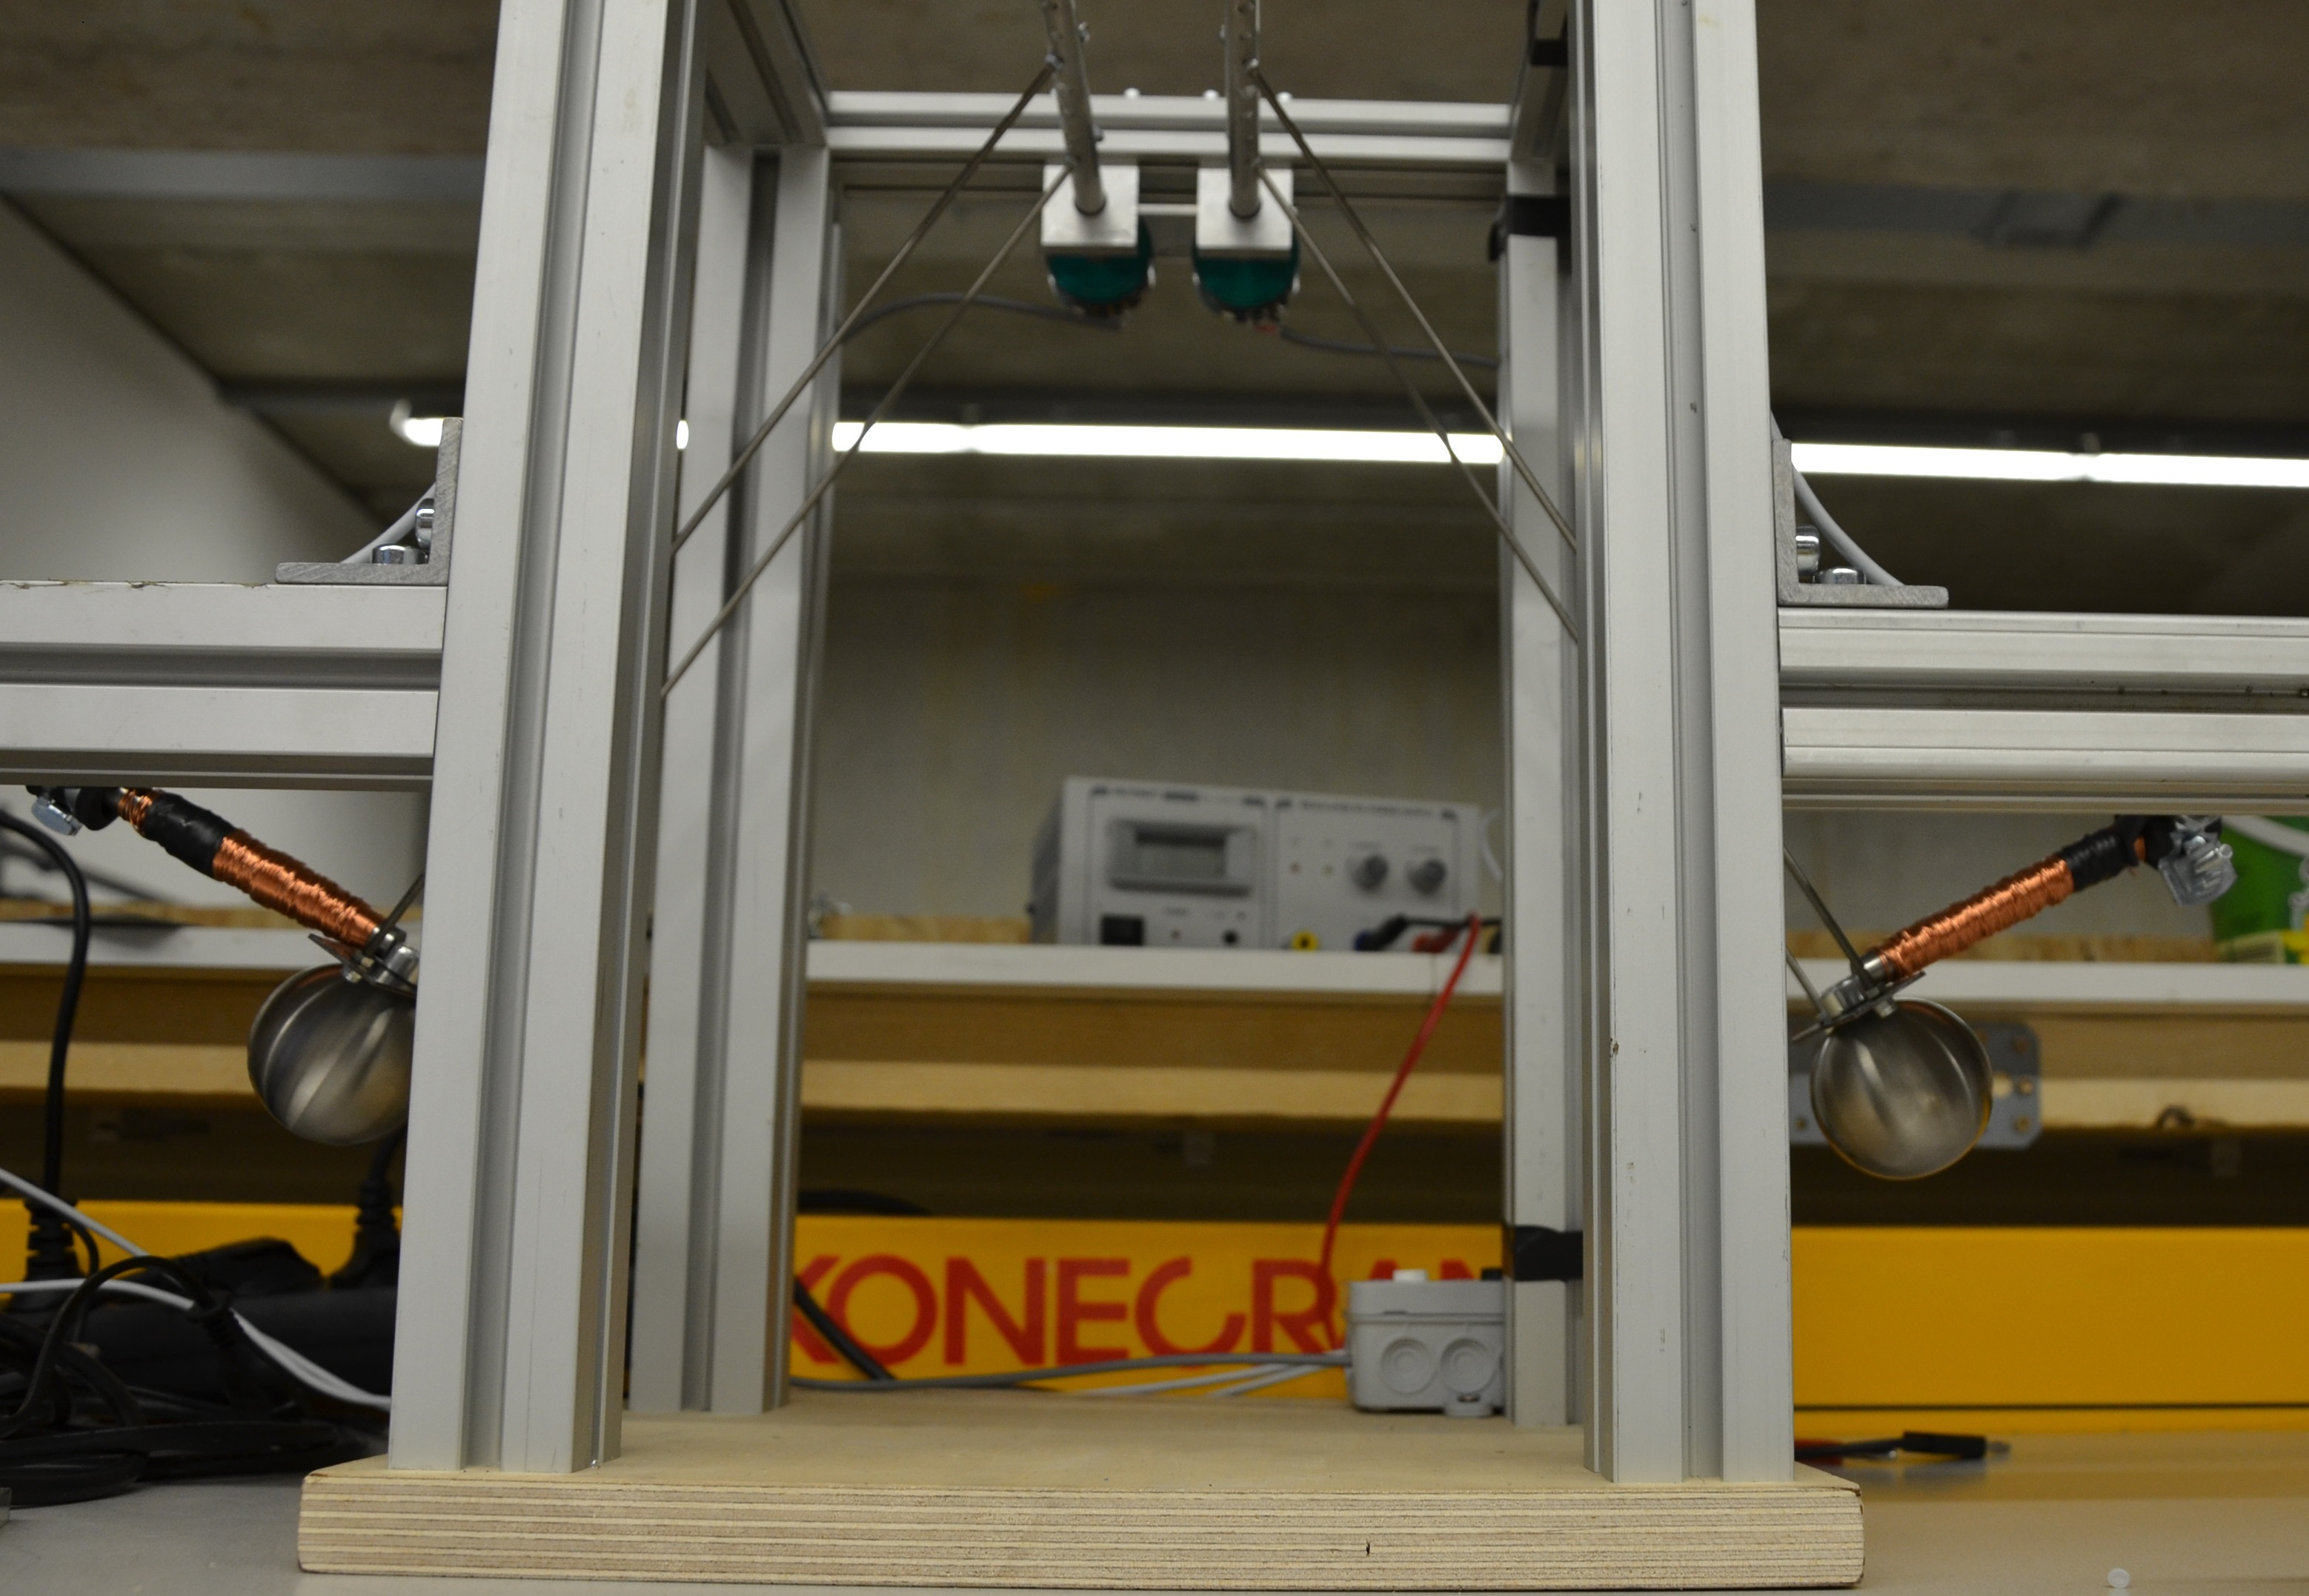
\includegraphics[width=.48\columnwidth]{007hollowspheredevice2}}  \quad
\subfloat[Coefficient of restitution of 2 mm silibeads]
{\label{fig:008esilibeads2mm2}%
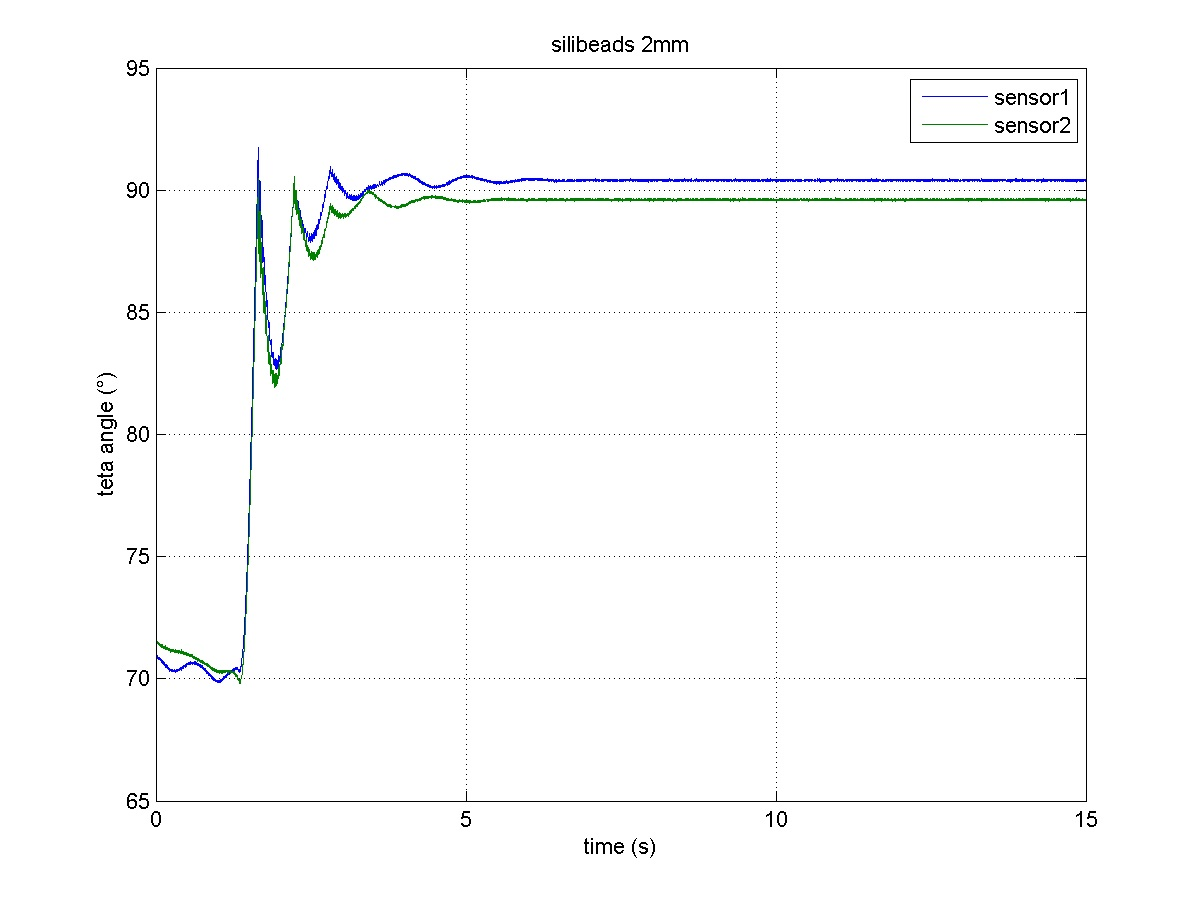
\includegraphics[width=.48\columnwidth]{008esilibeads2mm2}} \\
\caption[Hollow Spheres experiment]{Hollow Spheres experiment}
\label{fig:hollowspheres}
\end{figure}


Before start the spheres are kept at 40º from the vertical through magnetic rods, in order to avoid spin and torque when they are released.
After releasing the spheres move with a defined \ac{omega1}, calculated as the fraction of the angular displacement over time variation.
Then they collide and flee with an \ac{omega2}.\\

Now the results present little noise, as you can see in Figure \ref{fig:008esilibeads2mm2}.
Unfortunately the steel truss are transmitting vibration to the structure, I am trying to understand how much is the energy dissipation.\\

Soon I should receive a simulation script for this experiment.\\

%\subsubsection{HS}
%\label{subsubsection:hsexperiment}



%\subsubsection{HS simulation}
%\label{subsubsection:hssimulation}


%\input{Paragrafi/Newfloor}
%% !TEX encoding = UTF-8
% !TEX TS-program = pdflatex
% !TEX root = ../Articolo.tex
% !TEX spellcheck = it-IT

%************************************************
\section{Ipsum}
\label{sec:ipsum}
%************************************************


Lorem ipsum dolor sit amet, consectetuer adipiscing elit. Nam dui ligula, fringilla a, euismod sodales, sollicitudin vel, wisi. Morbi auctor lorem non justo. Nam lacus libero, pretium at, lobortis vitae, ultricies et, tellus.
\begin{description}
\item[Lorem ipsum dolor] sit amet, consectetuer adipiscing elit. Ut purus elit, vestibulum ut, placerat ac $\lim_{n \to \infty}\sum_{k=1}^n \frac{1}{k^2}= \frac{\pi^2}{6}$.
\item[Mauris ut leo.]
Cras viverra metus rhoncus sem. Nulla et lectus vestibulum urna fringilla ultrices. Phasellus eu tellus sit amet tortor gravida placerat.
\[
\lim_{n \to \infty}\sum_{k=1}^n \frac{1}{k^2}= \frac{\pi^2}{6}.
\]
\end{description}

Nulla malesuada porttitor diam. Donec felis erat, congue non, volutpat at, tincidunt tristique, libero. Vivamus viverra fermentum felis.
\begin{equation}
\label{eq:euler}
e^{i\pi}+1=0.
\end{equation}
Dalla formula~\eqref{eq:euler} 
si deduce che\dots






\subsection{Nozioni basilari}

\subsubsection{Insiemi numerici}

Donec nonummy pellentesque ante. Phasellus adipiscing semper elit.
\begin{equation}
x^2 \geq 0 \quad
\forall x \in \mathbb{R}.
\end{equation}


\subsubsection{Le matrici}

\lipsum[2]
\begin{equation}
A=
\begin{bmatrix}
x_{11} & x_{12} & \dots \\
x_{21} & x_{22} & \dots \\
\vdots & \vdots & \ddots
\end{bmatrix}
\end{equation}



\subsection{Formule fuori corpo}

Proin fermentum massa ac quam. Sed diam turpis, molestie vitae, placerat a, molestie nec, leo. Maecenas lacinia. Nam ipsum ligula, eleifend at, accumsan nec, suscipit a, ipsum. 


\subsubsection{Una formula spezzata con allineamento}

\lipsum[2]
\begin{equation} 
\begin{split} 
a &= b+c-d \\ 
  &= e-f \\ 
  &= g+h \\ 
  &= i. 
\end{split} 
\end{equation}

 
\subsubsection{Casi}

\lipsum[3]
\begin{equation}
f(n):=
\begin{cases} 
2n+1, & \text{con $n$ dispari,} \\ 
n/2,  & \text{con $n$ pari.} 
\end{cases} 
\end{equation}



\subsection{Enunciati e dimostrazioni}

Nunc eleifend consequat lorem. Sed lacinia nulla vitae enim. Pellentesque tincidunt purus vel magna. Integer non enim. Praesent euismod nunc eu purus.
\begin{definizione}[di Gauss] 
Un \emph{matematico} trova ovvio che
$\int_{-\infty}^{+\infty}
e^{-x^2}\,dx=\sqrt{\pi}$. 
\end{definizione} 
\begin{teorema} 
I matematici, se ce ne sono, sono molto rari.
\end{teorema} 

\lipsum[2]

\begin{teorema}[di Pitagora]
La somma dei quadrati costruiti sui cateti uguaglia il quadrato costruito sull'ipotenusa.
\end{teorema}
La dimostrazione viene lasciata per esercizio.

Donec bibendum quam in tellus. Nullam cursus pulvinar lectus. Donec et mi. Nam vulputate metus eu enim. Vestibulum pellentesque felis eu massa.
\begin{teorema}[Sorpresa]
Si ha che $\log(-1)^2=2\log(-1)$.
\end{teorema} 
\begin{proof} 
Si ha che $\log(1)^2 = 2\log(1)$.
Ma si ha anche che $\log(-1)^2=\log(1)=0$.
Quindi $2\log(-1)=0$, da cui la tesi.
\end{proof}
Viene un quadratino a fine dimostrazione.
\begin{legge}
\label{lex:capo}
Il capo ha ragione.
\end{legge}
\begin{decreto}[Aggiornamento alla legge~\ref{lex:capo}]
Il capo ha \emph{sempre} ragione.
\end{decreto}
\begin{legge}
Se il capo ha torto, vedere la 
legge~\ref{lex:capo}.
\end{legge}


Nam dui ligula, fringilla a, euismod sodales, sollicitudin vel, wisi. Morbi auctor lorem non justo. Nam lacus libero, pretium at, lobortis vitae, ultricies et, tellus.
\begin{murphy}
Cras nec ante. Pellentesque a nulla. Cum sociis natoque penatibus et magnis dis parturient montes, nascetur ridiculus mus. Aliquam tincidunt urna.
\end{murphy}

%\input{Paragrafi/trota}
\appendix
%% !TEX encoding = UTF-8
% !TEX TS-program = pdflatex
% !TEX root = ../Articolo.tex
% !TEX spellcheck = it-IT

%************************************************
\section{Dolor}
\label{sec:dolor}
%************************************************

\lipsum[1]

\subsection{Mane}
\lipsum[2]

\subsection{Tekel}
\lipsum[3]

\subsection{Fares}
\lipsum[4-5]

% *****************************************************************
% Materiale finale
%% !TEX encoding = UTF-8
% !TEX TS-program = pdflatex
% !TEX root = ../Articolo.tex
% !TEX spellcheck = it-IT

%************************************************
\section{Acronyms list}
\label{sec:acro}
%************************************************
%*******************************************************
% Elenco degli acronimi
%*******************************************************

		
\begin{acronym}[TDMA]
%\acro{CDMA}{Code Division Multiple Access}
%\acro{GSM}{Global System for Mobile communication}
%\acro{NA}[\ensuremath{N_{\mathrm A}}]{Number of Avogadro\acroextra{ (see \S\ref{Chem})}}
%\acro{NAD+}[NAD\textsuperscript{+}]{Nicotinamide Adenine Dinucleotide}
%\acro{NUA}{Not Used Acronym}
%\acro{TDMA}{Time Division Multiple Access}
%\acro{UA}{Used Acronym}
%\acro{lox}[\ensuremath{LOX}]{Liquid Oxygen}%
%\acro{lh2}[\ensuremath{LH_2}]{Liquid Hydrogen}%
%\acro{IC}{Integrated Circuit}%
%\acro{BUT}{Block Under Test}%
%\acrodefplural{BUT}{Blocks Under Test}%

\acro{phis}[$\phi_s$]{angle of sliding friction}
\acro{aor}[$AOR$]{Angle of repose}
\acro{omega1}[$\omega_1$]{angular speed before first impact}
\acro{omega2}[$\omega_2$]{angular speed after first impact}
\acro{omega3}[$\omega_3$]{angular speed before second impact}
\acro{omega4}[$\omega_4$]{angular speed after second impact}
\acro{dem}[$DEM$]{Discrete Element Method}
\acro{euno}[$e_1$]{coefficient of first restitution}
\acro{cor}[$COR$]{coefficient of restitution}
\acro{edue}[$e_2$]{coefficient of second restitution}
\acro{mu}[$\mu_s$]{coefficient of sliding friction}
\acro{mur}[$\mu_r$]{coefficient of static rolling friction}
\acro{jsct}[$JSCT$]{Jenike Shear Cell tester}
\acro{pmsct}[$PMSCT$]{``Poor Man'' Shear Cell tester}
\acro{liggghts}[$LIGGGHTS$]{LAMMPS improved for general granular and granular heat transfer simulations}
\acro{r}[$r$]{radius of the particle}
\acro{ra}[$R$]{external radius of the sphere}
\acro{sasct}[$SASCT$]{Schulze Annular Shear Cell tester}

\end{acronym}

% !TEX encoding = UTF-8
% !TEX TS-program = pdflatex
% !TEX root = ../Articolo.tex
% !TEX spellcheck = it-IT

%*******************************************************
% Bibliografia
%*******************************************************
%\nocite{*}
\printbibliography
%******************************************************************
\end{document}


